% tipo de documento y paquetes a utilizar.
\documentclass[12pt]{article}
\usepackage[utf8]{inputenc}
% \usepackage{amsmath, amsthm, amsfonts, mathtools} % Paquete para usar más fórmulas y ecuaciones.
\usepackage{graphicx}       % Paquete para usar imágenes y figuras.
\usepackage{geometry}       % Paquete para trabajar con los márgenes del documento.
\usepackage{fancyhdr}       % Paquete para personalizar encabezado y pie de página.
\usepackage{lastpage}       % Paquete para referenciar páginas del documento.
\usepackage{listings}       % Paquete para escribir código de programación.
\usepackage{inconsolata}    % Paquete de tipo de letra consola.
\usepackage{multirow}       % Paquete para combinar filas y columnas en tablas.
\usepackage{array}          % Paquete para trabajar tablas especializadas.
\usepackage{xcolor}         % Paquete básico para agregar color al texto.
\usepackage{float}          % Paquete para utilizar fijación de figuras H.
\usepackage{hyperref}       % Paquete para insertar links en el documento.

% Define colores nuevos.
\definecolor{color}{HTML}{E4E4EE}
\definecolor{verde}{HTML}{3C8031}

% Personalización de la fuente para el código.
\lstset{
    % language = C++,                       % Lenguaje con palabras reservadas de este resaltadas.
    basicstyle = \ttfamily\footnotesize,    % Utiliza la fuente tttfamily, en especial el paquete inconsolata.
    frame = single,                         % Quita el marco al cuadro flotante que contiene el código o texto.
    backgroundcolor = \color{color},        % Cambia el color del fondo del marco del código. Utiliza el paquete "xcolor" y define un nuevo color.
    columns = fullflexible,                 % Ajusta el cuadro flotante al tamaño del texto del documento.
    breaklines = true,                      % Ajusta el texto dentro del contenedor.
    inputencoding = utf8,                   % Admite caracteres del código UTF8.
    extendedchars = true,                   % Soporte para caracteres especiales.
    %numbers = left,                        % Agrega número de línea al código (izquierda, sin número y derecha).
    showstringspaces = false,               % Quita los guiones bajos predeterminados de los espacios en cadenas de texto.
    escapebegin = \obeyspaces,              % Complemento de la entrada anterior.
    % numberstyle = \color{red},            % Color de los números en el texto o código.
    % stringstyle = \color{red},            % Color de las cadenas de texto en el texto o código.
    % keywordstyle = \color{red},           % Color de las palabras reservadas en el texto o código.
    % identifierstyle = \color{red},        % Color del texto o código.
    commentstyle = \color{verde},           % Color de los comentarios en el texto o código.
    literate =                              % Acepta los siguientes caracteres especiales fuera de UTF8.
        {á}{{\'a}}1 {é}{{\'e}}1 {í}{{\'i}}1 {ó}{{\'o}}1 {ú}{{\'u}}1
        {Á}{{\'A}}1 {É}{{\'E}}1 {Í}{{\'I}}1 {Ó}{{\'O}}1 {Ú}{{\'U}}1
        {ñ}{{\~n}}1 {Ñ}{{\~N}}1,
}

% Márgenes del documento.
\newgeometry{
    top=2.5cm,     % Superior.
    bottom=2.5cm,  % Inferior.
    outer=2.5cm,   % Parte exterior.
    inner=2.5cm,    % Parte interior.
}

% Personalización de la cabecera y pie de página.
\pagestyle{fancy}
\fancyhf{}
\rhead{Overleaf}                                            % Texto en esquina superior derecha.
\lhead{Apuntes de JavaScript}                               % Texto en esquina superior izquierda.
\rfoot{Pagina \thepage \hspace{1pt} de \pageref{LastPage}}  % Texto en esquina inferior derecha (Página n de n).
% Ancho de línea horizontal superior e inferior.
\renewcommand{\headrulewidth}{1pt}
\renewcommand{\footrulewidth}{1pt}

% Datos para la portada del documento.
\title{Apuntes de JavaScript}
\author{migueluisV}
\date{Realizadas: Noviembre 2022}

% Inicio del documento.
\begin{document}

% Cambia los títulos de los índices:
% Content - Índice
% List of Figures - Índice de Figuras
% List of Tables - Índice de Tablas
\renewcommand*\contentsname{Índice}
\renewcommand{\listtablename}{Índice de Tablas}
\renewcommand{\listfigurename}{Índice de Figuras}

% Inserta la portada y los índices.
\maketitle\newpage
\tableofcontents\newpage
\listoffigures\newpage
\listoftables\newpage

% Incluye los archivos que conforman al proyecto.
\section{Conceptos básicos}

\textbf{JavaScript} es uno de los lenguajes de programación más populares, utilizado popularmente para crear sitios web dinámicos e interactivos, pero también es usado para crear aplicaciones de celular, videojuegos, procesamiento de datos y más.


\subsection{Salidas}

\textbf{Dentro de un documento HTML}

Una cosa es desplegar un mensaje en un archivo \textit{.js} y otra en un archivo \textit{.html}, con la función \textbf{document.write()} escribimos una cadena dentro de la etiqueta \textbf{<script>} en un archivo HTML.
\begin{lstlisting}
    <script>
        document.write("Hola mundo.")
    </script>
\end{lstlisting}

Gracias a que estamos escribiendo por medio del lenguaje de etiquetas HTML, podemos aplicar etiquetas del mismo al acabado de nuestro mensaje:
\begin{lstlisting}
    <script>
        <!- El mensaje estará escrito en negrita y cursiva. ->
        document.write("<br><i>Hola mundo.</i></br>")
    </script>
\end{lstlisting}

\textit{Nota}: es recomendable utilizar esta función únicamente para salidas de pruebas u errores.

\textbf{En la consola del buscador}

Para escribir un mensaje en la consola del navegador, utiliza el comando \textbf{console.log()}, el \textbf{texto} que vaya a ser escrito debe estar encerrado \textbf{entre comillas sencillas o dobles} ('texto', "texto").
\begin{lstlisting}
    \console.log("Esto es un mensaje.")
\end{lstlisting}

Este tipo de salida es más utilizada para pruebas y probar el funcionamiento del código, se recomienda esta función contra la mencionada anteriormente.


\subsection{Variables}

Para declarar una variable se utiliza la palabra reservada \textbf{var}:
\begin{lstlisting}
    var x = 10;
\end{lstlisting}

\textit{Nota}: JavaScript diferencia variables con el mismo nombre pero distinta cantidad de variables, "nombre" y "Nombre" son dos variables distintas.

Algunas reglas para la declaración de variables en este lenguaje son:
\begin{enumerate}
    \item El primer carácter de una variable debe ser una letra, \textbf{guión bajo} (\_) o un \textbf{símbolo de dolar} (\$).
    \item El primer carácter de una variable no puede ser un número.
    \item Los nombres de variables no pueden incluir operadores matemáticos o lógicos.
    \item Los nombres de variables no pueden contener espacios en blanco.
    \item Los nombres de variables no pueden contener símbolos especiales (", \#, \%, \&, etc).
\end{enumerate}


\subsection{Comentarios}

Para comentar una sola línea de código se utilizan \textbf{dos diagonales} (\textbf{//}) y para comentar múltiples líneas se utiliza los caracteres \textbf{/*} al inicio de las instrucciones que buscas comentar, y \textbf{*/} al final de las instrucciones.
\begin{lstlisting}
    // Esto es un comentario.
    alert("Mensaje dentro de una alerta.")
    /*
    Esto
    También
    Es
    Un
    Comentario.
    */
\end{lstlisting}


\subsection{Tipos de datos}

En este lenguaje, no es necesario declarar una variable con su tipo de dato, sin embargo, no es una buena práctica declarar una variable con un entero, y algunas instrucciones después, asignarle una cadena de caracteres.
\begin{lstlisting}
    // Declaración de variables.
    var x = 1;
    var y = 1.1;
    var z = 1.1111;
    x = "Esto es una variable"; // Esto no es correcto.
\end{lstlisting}

Podemos utilizar una sola comilla (') o dobles comillas (") para contener un texto dentro de una variable, a su vez, podemos utilizar los escapes \textbackslash " y \textbackslash ' para utilizar dichas comillas dentro de una cadena.
\begin{lstlisting}
    var nombre = "mi nombre es \"mario\"";
    var apellido = 'mi nombre es \'casas\''
    var edad = "mi edad es '21'";
\end{lstlisting}

\textit{Nota}: no es necesario utilizar caracteres de escape de una comilla dentro de dobles comillas, ni dobles comillas dentro de comillas.

Algunos caracteres de escape que podemos utilizan se ven en la \textit{Tabla \ref{tab: 1}}:
\begin{table}[H]
    \begin{center}
        \caption{Caracteres de escape válidos}
        \label{tab: 1}
        \begin{tabular}{c l}
            \hline
            \textbf{Carácter de escape}&\textbf{Función} \\
            \hline
            \textbackslash ' & Una comilla \\
            \textbackslash " & Doble comilla \\
            \textbackslash \textbackslash & Diagonal \\
            \textbackslash n & Salto de línea \\
            \textbackslash r & Posiciona el cursor al inicio de la línea \\
            \textbackslash t & Tabulación \\
            \textbackslash b & Posiciona el cursos un carácter atrás en el texto o consola \\
            \textbackslash f & Genera un salto de página \\
            \hline
        \end{tabular}
    \end{center}
\end{table}

Los \textbf{valores booleanos} son: \textbf{true} y \textbf{false}, el primero para casos positivos o reales, el segundo para valores como 0, null, indefinido o cadenas vacías.


\subsection{Operadores}


\subsubsection{Operadores aritméticos}

La \textit{Tabla \ref{tab: 2}} contiene los operadores aritméticos válidos en este lenguaje:
\begin{table}[H]
    \begin{center}
        \caption{Operadores aritméticos en JavaScript}
        \label{tab: 2}
        \begin{tabular}{c l}
            \hline
            \textbf{Operador}&\textbf{Definición} \\
            \hline
            + & Suma o Concatenación \\
            - & Resta \\
            $\ast$ & Multiplicación \\
            / & División \\
            \% & Modulo (residuo de una división) \\
            ++ & Incremento \\
            -- & Decremento \\
            \hline
        \end{tabular}
    \end{center}
\end{table}

La función \textbf{eval()} toma una cadena que contiene una expresión aritmética y regresa su resultado:
\begin{center}
    \textit{console.log(eval("2 + 2")); // Imprime 4.}
\end{center}

Al igual que en otros lenguajes, JavaScript posee los operadores de incremento y decremento post y pre:
\begin{center}
    \textit{
            var++ (incrementa después de una instrucción) \\
            ++var (incrementa antes de una instrucción) \\
            var-- (decrementa después de una instrucción) \\
            --var (decrementa antes de una instrucción) \\
    }
\end{center}


\subsubsection{Operadores de asignación}

La \textit{Tabla \ref{tab: 3}} contiene los operadores de asignación válidos en este lenguaje:
\begin{table}[H]
    \begin{center}
        \caption{Operadores de asignación en JavaScript}
        \label{tab: 3}
        \begin{tabular}{c l}
            \hline
            \textbf{Operador}&\textbf{Equivalencia} \\
            \hline
            = & x = y \\
            += & x = x + y \\
            -= & x = x - y \\
            *= & x = x * y \\
            /= & x = x / y \\
            \%= & x = x \% y \\
            \hline
        \end{tabular}
    \end{center}
\end{table}

\textit{Nota}: pueden combinarse el uso de varios operadores de asignación en una sola instrucción.


\subsubsection{Operadores de comparación}

La \textit{Tabla \ref{tab: 4}} contiene los operadores de comparación válidos en este lenguaje:
\begin{table}[H]
    \begin{center}
        \caption{Operadores de comparación en JavaScript}
        \label{tab: 4}
        \begin{tabular}{c l}
            \hline
            \textbf{Operador}&\textbf{Definición} \\
            \hline
            == & Igual a \\
            === & Idénticos (iguales o del mismo tipo) \\
            != & No igual a \\
            !== & No idéntico \\
            $>$ & Mayor \\
            $>$= & Mayor igual \\
            $<$ & Menor \\
            $<$= & Menor igual \\
            \hline
        \end{tabular}
    \end{center}
\end{table}

Las comparaciones regresan true o false si son ciertas o no.


\subsubsection{Operadores lógicos y booleanos}

La \textit{Tabla \ref{tab: 5}} contiene los operadores lógicos válidos en este lenguaje:
\begin{table}[H]
    \begin{center}
        \caption{Operadores de comparación en JavaScript}
        \label{tab: 5}
        \begin{tabular}{m{3cm} m{10cm}}
            \hline
            \textbf{Operador}&\textbf{Definición} \\
            \hline
            \&\& & Y. Regresa true si ambas expresiones son verdaderas \\
            $||$ & O. Regresa true si una de las expresiones es verdadera \\
            ! & Negación. Regresa el valor contrario (true o false) al resultado de la expresión \\
            \hline
        \end{tabular}
    \end{center}
\end{table}

Este lenguaje soporta el uso del \textbf{operador ternario}:
\begin{lstlisting}
    var mayorDeEdad = (edad < 18) ? "Muy joven" : "Muy viejo";
\end{lstlisting}

Como vimos, está constituido de una condición, el símbolo de pregunta, su primer valor, dos puntos y el segundo valor; solamente soporta dos valores (true y false), a diferencia de una sentencia if, que puede tener varios \textit{if´s anidados} o \textit{else if}.
\begin{lstlisting}
    variable = (condición) ? valor1 : valor2
\end{lstlisting}

\section{Evaluación de expresiones}


\subsection{Sentencia if else}
Evalúa una expresión, si esta es acertada regresa true, si no lo es, regresa false. Su estructura es la siguiente:
\begin{lstlisting}
    if (condición) {
        // Código.
    }
    else {
        // Código.
    }
\end{lstlisting}

\textit{Nota}: el lenguaje soporta que, si solamente se escribe una instrucción en cualquiera de sus bloques, no sea necesario escribir las llaves y el bloque \textit{else} puede ser omitido.


\subsection{Sentencia else if}

En ocasiones, es requerido que se evalúe una condición si una condición previa fue falsa, para eso funciona la sentencia else if:
\begin{lstlisting}
    if (condición 1) {
        // Código.
    }
    else if (condición 2) {
        // Código.
    } else {
        // Código.
    }
\end{lstlisting}


\subsection{Sentencia switch}

Evalúa una variable y se le asigna un valor dependiendo de otra cantidad de valores o parámetros. Su estructura es la siguiente:
\begin{lstlisting}
    switch (variable o expresión) {
        case n1:
            // Código.
            break;
        case n2:
            // Código.
            break;
        .
        .
        .
        case n:
            // Código.
            break;
        default:
            // Código.
    }
\end{lstlisting}

\textit{Nota}: el valor \textbf{default} puede ser omitido y no es obligatoria la palabra reservada \textbf{break}.



\section{Ciclos}

\subsection{Ciclo For}

Ejecuta un bloque de código n cantidad de veces. Su estructura es:
\begin{lstlisting}
    for (inicializador o contador; condición para ejecución; incremento o decremento) {
        // Código.
    }
\end{lstlisting}

Donde:
\begin{itemize}
    \item \textbf{inicializador o contador}: es la variable que será incrementada o decrementada a lo largo de la ejecución del bloque de código. Puede ser omitido siempre y cuando haya alguna variable fuera de la declaración del ciclo que maneje la ejecución del mismo, a su vez, pueden haber múltiples contadores dentro de la declaración.
    \item \textbf{condición para ejecución}: condición que permite que el bloque se ejecute; si la condición ya no es cierta, se sale del ciclo.
    \item \textbf{incremento o decremento}: incrementa o decrementa la variable contador cuando una vuelta se da en el ciclo.
\end{itemize}

Vemos a continuación dos ejemplos del primer punto anterior mencionados:
\begin{lstlisting}
    i = 1;
    // Ciclo for sin un contador.
    for (; i < 5; i++) {}
    // Ciclo for con dos contadores o inicializadores.
    for (x = 1, text = ""; x < 5; x++) {}
\end{lstlisting}


\subsection{Ciclo While}

Ejecuta un bloque de código mientras una condición sea verdadera. Su estructura es:
\begin{lstlisting}
    while (condición) {
        // Código.
    }
\end{lstlisting}

Debe poseer una variable contador dentro de su bloque para manejar las vueltas dentro del ciclo y su fin es que el ciclo termine, sino, sería un ciclo infinito.


\subsection{Ciclo Do-While}

Ejecuta un bloque de código mientras una condición sea verdadera y se ejecuta mínimo una vez. Su estructura es:
\begin{lstlisting}
    do {
        // Código.
    }
    while (condición);
\end{lstlisting}


\subsection{Break y Continue}

La palabra reservada \textbf{break} es utilizada para terminar la ejecución de un ciclo, aún si su condición todavía era verdadera como para continuar con las vueltas.

La palabra reservada \textbf{continue} es utilizada para saltar n cantidad de líneas de código después de la palabra reservada en cuestión, es decir, salta una vuelta del ciclo. Veremos un ejemplo de ambas a continuación:
\begin{lstlisting}
    for (x = 1; x <= 10; x++) {
        if (x == 5){
            continue;
        }
        console.log(x);
        if (x == 8){
            break;
        }
    }

    /*
    Imprime:
    1
    2
    3
    4
    6
    7
    8
    */
\end{lstlisting}

En el código anterior se imprimen los primeros cuatro números, se salta el número cinco por la sentencia \textit{continue} y continua imprimiendo, cuando x vale ocho, termina el ciclo.

\section{Funciones}
\hspace{0.55cm}Una \textbf{función} es un bloque de código que realiza una tarea particular, esta tarea es ejecutada cuando se le "llama" a la función para que ejecute sus instrucciones. Su estructura es la siguiente:
\begin{lstlisting}
    function nombre (parámetros) {
        // Instrucciones.
    }
\end{lstlisting}

Los nombres de funciones siguen las mismas reglas que los nombres de variables. Las funciones se pueden llamar simplemente escribiendo su nombre, seguido por paréntesis o por un punto y la función \textbf{call()}:
\begin{lstlisting}
    function hola () {
        console.log("hola mundo")
    }

    hola()
    hola.call()
\end{lstlisting}


\subsection{Parámetros}
\hspace{0.55cm}Son valores que recibe la función y que pueden ser utilizados por la misma para realizar su tarea. Su estructura es la siguiente:
\begin{lstlisting}
    function nombre (parámetro1, parámetro2, ..., parámetroN) {
        // Instrucciones.
    }
\end{lstlisting}

En caso de que se llame a una función y no se le pasen la cantidad de parámetros que posee (se le pasan dos en vez de tres), aquellos que no recibieron un valor pasan a ser \textbf{undefined}. Vemos entonces que los parámetros, al igual que las variables, \textbf{no requieren de indicar su tipo de dato}.


\subsection{Sentencia return}
\hspace{0.55cm}La palabra reservada \textbf{return} es utilizada para regresar un valor de una función, una vez que el lenguaje encuentra esta palabra en una función, acaba la ejecución de la misma. Veamos un ejemplo:
\begin{lstlisting}
    function alCubo (num) {
        return num * num * num;
    }

    console.log(alCubo(3))
\end{lstlisting}

En caso de que haya un error regresando un valor o variable, o esta variable no tenga ningún valor, lo que regresará la funcioón es \textbf{undefined}.


\subsection{Funciones Alert, Prompt y Confirm}
\hspace{0.55cm}La función \textbf{alert()} muestra una caja con un mensaje en el sitio web, el único parámetro que recibe es una cadena, la cual muestra al usuario, y posee un único botón para interactuar, el cual dice OK, como se ve en la \textit{Figura \ref{fig: 1}}.
\begin{figure}[H]
    \caption{Ejemplo de la función alert()}
    \label{fig: 1}
    \begin{center}
        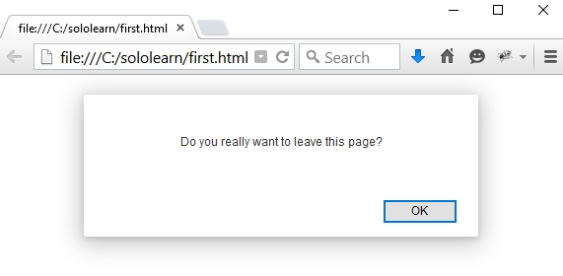
\includegraphics [width=9cm]{ss/alert.png}
    \end{center}
\end{figure}
La función \textbf{prompt()} muestra una caja con un mensaje en el sitio web, y solicita al usuario que ingrese alguna información; posee dos parámetros: el primero es el mensaje a mostrar en la caja y el segundo es un texto por defecto dentro de la caja de texto que posee la caja; posee dos botones: el botón OK, si es presionado, la función regresa lo que el usuario ingresó, y el botón Cancel, que cierra la caja y regresa null, como vemos en la \textit{Figura \ref{fig: 2}}. No se recomienda utilizar demasiado esta función.
\begin{figure}[H]
    \caption{Ejemplo de la función prompt()}
    \label{fig: 2}
    \begin{center}
        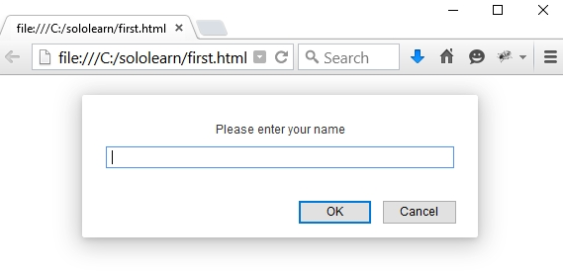
\includegraphics [width=9cm]{ss/prompt.png}
    \end{center}
\end{figure}
La función \textbf{confirm()} muestra una caja con un mensaje en el sitio web, muestra un mensaje que el usuario debe confirmar para continuar; esta caja posee dos botones: el botón OK, si es presionado, la función regresa true, y el botón Cancel, que cierra la caja y regresa false; la \textit{Figura \ref{fig: 3}} muestra como se ve inicialmente la caja de confirm().
\begin{figure}[H]
    \caption{Ejemplo de la función confirm()}
    \label{fig: 3}
    \begin{center}
        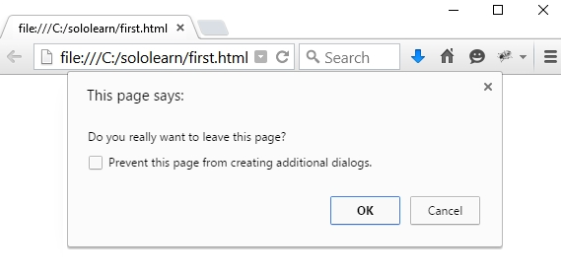
\includegraphics [width=9cm]{ss/confirm.png}
    \end{center}
\end{figure}
No es recomendado utilizar demasiado este método, porque impide que el usuario interactúe con el sitio hasta que de clic en alguno de los botones de la caja; la \textit{Figura \ref{fig: 4}} muestra la caja cuando se le da clic al botón OK.
\begin{figure}[H]
    \caption{Mensaje cuando se presiona botón OK de la función confirm()}
    \label{fig: 4}
    \begin{center}
        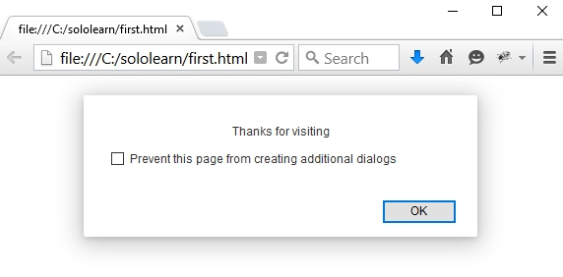
\includegraphics [width=9cm]{ss/confirm_res.png}
    \end{center}
\end{figure}


\subsection{Función setInterval}
\hspace{0.55cm}Esta función llama a una función o evalúa una expresión cada determinado tiempo (en milisegundos), seguirá llamando o evaluando hasta que se ejecute la función \textbf{clearInterval()}, como vemos enseguida:
\begin{lstlisting}
    // Declara función para mostrar en ventana un mensaje.
    function miAlerta() {
        alert("Hola mundo");
    }

    // Llama a la función setInterval que llama a la función miAlerta
    // cada tres segundos.
    setInterval(miAlerta, 3000);
\end{lstlisting}

Nótese que, dentro de los parámetros de \textit{setInterval()}, la función a llamar no posee paréntesis al final de su nombre. Para el caso anterior, la función setInterval no detendrá su ejecución porque no está la instrucción \textit{clearInterval()} ni aunque se presione el botón OK de la caja.
\section{Objetos}

Un objeto de JavaScript (JS para abreviar) es similar a un objeto de clase en otro lenguaje, es decir, un objeto JS puede ser un auto, con las propiedades de marca, modelo, kilometraje, número de llantas, el método de andar, reversa, acelerar, frenar, etc. Tienen el siguiente aspecto:
\begin{lstlisting}
    var objeto = {
        propiedad1: valor1,
        propiedad2: valor2.
        .
        .
        .
        propiedadN: valorN
    };
\end{lstlisting}

La creación de métodos de objetos se verá más adelante. Podemos ver las propiedades y sus valores como el contenido \textbf{pares llave-valor} de un contenedor.

Para acceder a las propiedades de un objeto JS utilizamos el operador punto (.) o las llaves cuadradas ([]):
\begin{lstlisting}
    // Declara objeto JS.
    var persona = {
        // Propiedades.
        nombre: "Luis",
        edad: 21,
        color_fav: "rojo",
        altura: 162
    };

    // Asigna propiedad del objeto JS a variable.
    var nom = persona.nombre;
    var nombre = persona["nombre"];

    document.write(nom);
    document.write(nombre);

    //Imprime: LuisLuis.
\end{lstlisting}

Con la función \textbf{length} podemos acceder a la cantidad de caracteres de una propiedad de un objeto JS.
\begin{lstlisting}
    // Asigna cantidad de caracteres de una propiedad del objeto JS a variable.
    var nom = persona.nombre.length;

    document.write(nom);

    //Imprime: 4.
\end{lstlisting}


\subsection{Creando objetos}

La forma de crear objetos vista anteriormente funciona únicamente para crear un solo objeto, se declara y se le asignan valores, pero no puedes tener más de un mismo tipo de objeto con la declaración previa.

Para tener una \textbf{plantilla de objetos} o un \textbf{tipo de objeto} (una clase de donde sacar los objetos en otros lenguajes vaya) utilizamos una \textbf{función constructor}:
\begin{lstlisting}
    // Declara objeto JS sin función constructor.
    var persona = {
        // Propiedades.
        nombre: "Luis",
        edad: 21,
        color_fav: "rojo",
        altura: 162
    };

    // Declara objeto JS con función constructor.
    function person(nombre, edad, peso) {
        // Asignación de valores a propiedades de objeto por medio de parámetros
        // y la palabra reservada "this".
        this.nombre = nombre;
        this.edad = edad;
        this.peso = peso;
    }
\end{lstlisting}

Así como con constructores en otros lenguajes, aquí creamos uno por medio de una función y se le asignan los valores a las propiedades por medio de parámetros, nótese que utilizamos la palabra reservada \textbf{this}, la cual asigna un valor al contexto en la que está contenida (la función person) y solo le pertenecerá a ese contexto ese valor. Ahora veamos como declarar varios objetos de la función constructor:
\begin{lstlisting}
    // Asigna declaración de objetos a variables.
    var p1 = new person("Daniela", 22, 50);
    var p2 = new person("Kevin", 26, 55);
\end{lstlisting}

Fíjese que se utiliza la palabra reservada \textbf{new} para declarar un objeto JS, esto diferencia a la declaración de objetos que ya habíamos previamente, porque esta palabra reservada hace que sea distinto un objeto declarado previamente a este nuevo que estamos creando. Con estos dos objetos declarados, podemos acceder a sus propiedades por el operador punto o llaves cuadradas.


\subsection{Métodos objetos}

Al igual que con las propiedades, para declarar un método de objeto se utiliza la palabra reservada \textbf{this} y para acceder al mismo se utiliza el operador punto o las llaves cuadradas; utilizamos una sintaxis particular:
\begin{lstlisting}
    // Declara objeto JS con función constructor.
    function person(nombre, edad, peso) {
        // Asignación de valores a propiedades de objeto por medio de parámetros
        // y la palabra reservada "this".
        this.nombre = nombre;
        this.edad = edad;
        this.peso = peso;
        // Declara método de objeto que cambia el peso y nombre del objeto.
        this.cambioNombrePeso = function(nombre, peso) {
            this.nombre = nombre;
            this.peso = peso;
        }
    }

    // Asigna declaración de objetos a variable.
    var p1 = new person("Daniela", 22, 50);
    // Llamada a método de objeto.
    p1.cambioNombrePeso("Gabriela", 49)
\end{lstlisting}

La estructura que se siguió es la siguiente:
\begin{lstlisting}
    nombreObjeto = function(parámetros) {
        // Código.
    }
\end{lstlisting}

Se pueden declarar métodos fuera de la declaración de un objeto JS y asignarle el método exterior a un método interno del objeto, como vemos a continuación:
\begin{lstlisting}
    // Declara objeto JS con función constructor.
    function person(nombre, edad, peso) {
        // Asignación de valores a propiedades de objeto por medio de parámetros
        // y la palabra reservada "this".
        this.nombre = nombre;
        this.edad = edad;
        this.peso = peso;
        // Declara método de objeto que cambia el peso y nombre del objeto
        // y se le asigna un método exterior.
        this.cambioNombrePeso = cambiarNombrePeso;
        }
    }
    
    // Función exterior asignada a método de objeto.
    function cambioNombrePeso(nombre, peso) {
        this.nombre = nombre;
        this.peso = peso;
    }
\end{lstlisting}

\textit{Nota}: nótese que, al asignar un método exterior a un método de objeto, el método exterior no requiere de paréntesis.


\subsection{Objeto Math}

Este \textbf{objeto} posee propiedades y métodos para realizar algunas operaciones matemáticas. La \textit{Tabla \ref{tab: 6}} almacena las propiedades del objeto:
\begin{table}[H]
    \begin{center}
        \caption{Propiedades del objeto Math}
        \label{tab: 6}
        \begin{tabular}{c l}
            \hline
            \textbf{Método}&\textbf{Definición} \\
            \hline
            E & Constante Euler \\
            LN2 & Logaritmo natural de 2 \\
            LN10 & Logaritmo natural de 10 \\
            LOG2E & Logaritmo base 2 de la constante Euler \\
            LOG10E & Logaritmo base 10 de la constante Euler \\
            PI & Constante PI \\
            \hline
        \end{tabular}
    \end{center}
\end{table}

La \textit{Tabla \ref{tab: 7}} almacena los métodos más utilizados del objeto:
\begin{table}[H]
    \begin{center}
        \caption{Métodos del objeto Math}
        \label{tab: 7}
        \begin{tabular}{m{4cm} m{9cm}}
            \hline
            \textbf{Método}&\textbf{Definición} \\
            \hline
            sqrt(x) & Regresa la raíz cuadrada de un valor \\
            round(x) & Regresa un valor decimal redondeado a su entero más cercano \\
            random() & Regresa un valor aleatorio entre 0 y 1 \\
            pow(x, y) & Regresa un número elevado a \textit{n} potencia \\
            min(x, y, z, ..., n) & Regresa el valor más pequeño de entre un conjunto \\
            max(x, y, z, ..., n) & Regresa el valor más grande de entre un conjunto \\
            abs(x) & Regresa el valor absoluto de un número \\
            \hline
        \end{tabular}
    \end{center}
\end{table}

Este objeto se utiliza de la siguiente manera:
\begin{lstlisting}
    var res = Math.sqrt(4);
    document.write(Math.PI + " " + res);

    // Imprime: 3.141592653589793.
\end{lstlisting}


\subsubsection{Números aleatorios entre un rango de números}

En caso de que necesitemos un número aleatorio entre 5 y 10, utilizamos el siguiente código:
\begin{lstlisting}
    function aleatorioEntero(min, max) {
        min = Math.ceil(min);
        max = Math.floor(max);
        return Math.floor(Math.random() * (max - min) + min);
}
\end{lstlisting}

La función regresa un número entero dentro de un rango de valores, la función está hecha de tal forma que, si el número máximo o mínimo es un decimal, este lo convierte a un número entero, y si ya es entero lo mantiene (\textit{líneas 2 y 3 del código}), posterior a ello, realiza el cálculo del número aleatorio (\textit{l código}). Esta función \textbf{incluye el número mínimo y excluye el mayor}; si deseamos que incluya tanto el número mínimo como máximo, cambiemos ligeramente la función a:
\begin{lstlisting}
    function aleatorioEntero(min, max) {
        min = Math.ceil(min);
        max = Math.floor(max);
        return Math.floor(Math.random() * (max - min + 1) + min);
}
\end{lstlisting}

Las dos funciones aplican a números enteros, si queremos un número aleatorio decimal entre un rango de valores, quitamos las líneas de código 2 y 3 para ambos casos:

\begin{lstlisting}
    function aleatorioEntero(min, max) {
        return Math.floor(Math.random() * (max - min + 1) + min);
}
\end{lstlisting}

El número retornado tendrá una gran cantidad de decimales.


\subsection{Objeto Date}

Este objeto permite crear variables con una determinada fecha, la cual está compuesta por:
\begin{itemize}
    \item año,
    \item mes,
    \item día,
    \item hora,
    \item minutos,
    \item segundos,
    \item milisegundos (un número entero: 3 seg = 3000),
\end{itemize}

Tenemos nueve formas para declarar una fecha:
\begin{itemize}
    \item new Date(): almacena la fecha actual del navegador o sistema.
    \item new Date(cadena con la fecha): almacena la fecha escrita en una cadena, la cual sigue el formato \textit{"mes día, año hora:minuto:segundo:milisegundo"}.
    \item new Date(year, month): almacena una fecha con el año y mes.
    \item new Date(year, month, day): almacena una fecha con el año, mes y día.
    \item new Date(year, month, day, hours): almacena una fecha con el año, mes, día y hora.
    \item new Date(year, month, day, hours, minutes): almacena una fecha con el año, mes, día, hora y minuto.
    \item new Date(year, month, day, hours, minutes, seconds): almacena una fecha con el año, mes, día, hora, minuto y segundos.
    \item new Date(year, month, day, hours, minutes, seconds, miliseconds): almacena una fecha con el año, mes, día, hora, minuto, segundos y milisegundos.
    \item new Date(miliseconds): almacena una fecha calculada a partir de los milisegundos.
\end{itemize}

El lenguaje tiene una fecha inicial, la cual es el \textbf{01 de enero de 1970, con hora 00:00:00}, en zona horaria \textbf{Tiempo Universal (UTC: Universal Time en inglés)}, con esta información se calcula una fecha cuando le pasas una cantidad de milisegundos; \textbf{los meses se cuentan a partir del cero} (0-11) y \textbf{los días a partir del uno} (1-31, 1-30); para terminar, \textbf{los objetos Date son estáticos}, quiere decir que una vez declarados, el tiempo en la máquina en el navegador sigue corriendo, pero el tiempo almacenado en el objeto ya no cambia.


\subsubsection{Métodos}

La \textit{Tabla \ref{tab: 8}} contiene los métodos disponibles de los objetos Date:
\begin{table}[H]
    \begin{center}
        \caption{Métodos del objeto Date}
        \label{tab: 8}
        \begin{tabular}{c l}
            \hline
            \textbf{Método}&\textbf{Definición} \\
            \hline
            getFullYear() & Regresa el año de una fecha \\
            getMonth() & Regresa el mes de una fecha \\
            getDate() & Regresa el día del mes de una fecha \\
            getDay() & Regresa el día de la semana de una fecha \\
            getHours() & Regresa la hora de una fecha \\
            getMinutes() & Regresa el minuto de una fecha \\
            getSeconds() & Regresa el segundo de una fecha \\
            getMiliseconds() & Regresa el milisegundo de una fecha \\
            \hline
        \end{tabular}
    \end{center}
\end{table}



\section{Objetos JSON}

JavaScript Object Notation (JSON) es un formato basado en texto estándar para representar datos estructurados en la sintaxis de objetos de JavaScript. Es comúnmente utilizado para transmitir datos en aplicaciones web (por ejemplo: enviar algunos datos desde el servidor al cliente, así estos datos pueden ser mostrados en páginas web, o vice versa). Aunque es muy parecido a la sintaxis de objeto literal de JavaScript, puede ser utilizado independientemente de JS, muchos entornos de programación poseen la capacidad de leer y generar JSON, tome en cuenta las siguientes consideraciones:
\begin{itemize}
    \item \textbf{Convertir} un objeto JSON a JS es llamado \textit{parsing}.
    \item \textbf{Convertir} un objeto JS  a JSON es llamado \textit{stringfy} o \textit{stringfication}.
    \item JSON solamente contiene propiedades, \textbf{no métodos}.
    \item JSON no acepta comillas simples ('') para la declaración de cadenas, solamente comillas dobles ("").
    \item JSON requiere que sus propiedades estén encerradas entre comillas.
\end{itemize}

Los JSON son cadenas - útiles cuando se quiere transmitir datos a través de una red. Debe ser convertido a un objeto nativo de JavaScript cuando se requiera acceder a sus datos. Ésto no es un problema, dado que JavaScript posee un objeto global JSON que tiene los métodos disponibles para convertir entre ellos. un objeto JSON puede ser almacenado en su propio archivo con extensión \textit{.json}, y en el archivo principal se importa con una \textbf{MIME type} de \textit{directorio/archivo .json}.


\subsection{Estructura}

Los objetos JSON es una cadena que sigue la estructura o lógica de los objetos JS, sin embargo, estos también pueden contener tipos de datos de JavaScript (enteros, punto flotante, booleanos, arreglos y otros objetos). Veamos el aspecto que tiene un objeto JSON:
\begin{lstlisting}
    {
        "squadName": "Super hero squad",
        "homeTown": "Metro City",
        "formed": 2016,
        "secretBase": "Super tower",
        "active": true,
        "members": [
            {
                "name": "Molecule Man",
                "age": 29,
                "secretIdentity": "Dan Jukes",
                "powers": [
                    "Radiation resistance",
                    "Turning tiny",
                    "Radiation blast"
                ]
            },
            {
                "name": "Madame Uppercut",
                "age": 39,
                "secretIdentity": "Jane Wilson",
                "powers": [
                    "Million tonne punch",
                    "Damage resistance",
                    "Superhuman reflexes"
                ]
            },
            {
                "name": "Eternal Flame",
                "age": 1000000,
                "secretIdentity": "Unknown",
                "powers": [
                    "Immortality",
                    "Heat Immunity",
                    "Inferno",
                    "Teleportation",
                    "Interdimensional travel"
                ]
            }
        ]
    };
\end{lstlisting}

Si deseamos acceder al contenido del objeto JSON en JavaScript, debemos \textit{parsearlo} y asignarlo a una variable del mismo nombre (para evitar confusión):
\begin{lstlisting}
    superHeroes.homeTown;
    superHeroes['active'];
\end{lstlisting}

Vemos que el ejemplo posee una propiedad que contiene varios elementos (arreglo), y dentro de estos elementos hay más propiedades que poseen aún más elementos (arreglos dentro de arreglos), podemos acceder a ellos de la siguiente manera:
\begin{lstlisting}
    superHeroes['members'][1]['powers'][2];
\end{lstlisting}



\section{Arreglos}

Para crear un arreglo en este lenguaje, se sigue la siguiente sintaxis:
\begin{center}
    \textit{var nombreArreglo = new Array(elementos);}
\end{center}

Para acceder a los elementos o modificar el valor de alguno de un arreglo, utilizamos los paréntesis cuadrados ([]) y el índice del elemento que deseemos (empezando de 0):
\begin{lstlisting}
    // Declara arreglo.
    var cursos = new Array("HTML", "CSS", "JS");
    // Imprime elemento en el índice 0 del arreglo.
    console.log(cursos[0]);
    // Cambiar el valor del elemento en el índice 0.
    cursos[0] = "C++";
    // Imprime elemento en el índice 0 del arreglo.
    console.log(cursos[0]);
\end{lstlisting}

En caso de que se desee acceder a un elemento en un índice inexistente de un arreglo, lo que regresará o mostrará el lenguaje es \textbf{undefined}.

Otra forma de declarar un arreglo (que es la forma en la cual suele hacerse) es de la siguiente manera:
\begin{center}
    \textit{var nombreArreglo = [elementos]}
\end{center}

Para accesar a sus elementos se hace de la misma manera que ya hemos visto.


\subsection{Inicialización de arreglos y arreglos dinámicos}

Por defecto, los arreglos del lenguaje son \textbf{dinámicos}, quiere decir que no requieren de una cantidad de elementos tope en su declaración y se pueden agregar cuantos elementos necesitemos, sin embargo, en la declaración de arreglos podemos asignarle un número tope si lo requerimos y asignarle elementos por separado o inicializado, como vemos enseguida:
\begin{lstlisting}
    // Declara arreglo inicializado.
    var numeros = [1, 2, 3, 4, 5];
    // Declara arreglo sin inicializar con tres elementos.
    var nombres = new Array(3);
    // Asigna elementos al arreglo.
    nombres[0] = "Luis";
    nombres[1] = "Daniela";
    nombres[2] = "Kevin";
    // Declara arreglos sin inicializar.
    var arboles = new Array();
    var autos = [];
\end{lstlisting}


\subsection{Métodos y propiedades}

Algunas funciones básicas de arreglos son:
\begin{itemize}
    \item \textbf{length}: regresa la cantidad de elementos que tiene un arreglo.
    \begin{center}
        \textit{arr.length}
    \end{center}
    \item \textbf{concat(arreglo)}: crea un nuevo arreglo a partir de otros dos.
    \begin{center}
        \textit{var arr3 = arr1.concat(arr2)}
    \end{center}
\end{itemize}


\subsection{Arreglos asociativos}

Otros lenguajes de programación poseen \textbf{arreglos asociativos}, los cuales utilizan palabras o nombres como índices, en vez de números, JavaScript no soporta este tipo de arreglos, pero pueden ser simulados utilizando los objetos que ya hemos visto:
\begin{lstlisting}
    // Declara arreglo sin inicializar.
    var persona = [];
    // El arreglo en el índice "nombre" se le asigna el valor "Luis".
    persona["nombre"] = "Luis";
    // El arreglo en el índice "edad" se le asigna el valor 21.
    persona["edad"] = 21;
    document.write(persona["edad"]);

    //Imprime: 21.
\end{lstlisting}

El arreglo es declarado como tal y vacío, pero los índices utilizados (nombre y edad) son de un objeto, es aspi que el arreglo es utilizado como un objeto, por lo cual, no se pueden utilizar los métodos de arreglos en objetos.

\section{DOM}

El \textbf{Modelo de Objetos de Documento} (\textbf{Documento Object Model}, abreviado DOM) es un modelo que contiene todos los objetos o estructura lógica de una página o sitio web.

Cuando el buscador busca acceder a un sitio web, primero carga toda la parte HTML de la misma para poder presentarlo en la pantalla, para lograr esto, construye el DOM del sitio, el cual puede ser representado o visualizado mejor en la \textit{Figura \ref{fig: 5}}:
\begin{figure}[H]
    \caption{Ejemplificación del DOM de HTML de un sitio web}
    \label{fig: 5}
    \begin{center}
        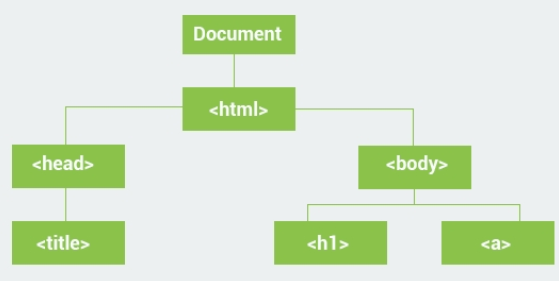
\includegraphics [width=9cm]{ss/dom_html.png}
    \end{center}
\end{figure}

Si refrescamos memoria, HTML se maneja por medio de etiquetas, una de apertura y una de cierre, dentro de las etiquetas podemos meter más etiquetas que cumplen con distintas funciones, lo que representa el DOM es esa jerarquía o árbol de etiquetas (ahora llamados \textbf{nodos}) que constituye un sitio web, que es lo que se ve en la imagen anterior (nodo raíz, hermanos, hijos, etc). En la previa imagen, tenemos que:
\begin{itemize}
    \item El nodo $<$html$>$ tiene dos hijos: $<$head$>$ y $<$body$>$.
    \item El nodo$<$head$>$ tiene un hijo: $<$title$>$.
    \item El nodo $<$title$>$ tiene un padre: $<$head$>$.
    \item El nodo $<$body$>$ tiene dos hijos: $<$h1$>$ y $<$a$>$.
    \item Los nodos $<$h1$>$ y $<$a$>$ tienen un padre: $<$body$>$:
    \item Los nodos $<$head$>$ y $<$body$>$ son hermanos o están al mismo nivel.
\end{itemize}

\textbf{JavaScript puede manipular el DOM de un sitio web} para volverlo dinámico y agregar, modificar o eliminar los nodos del DOM. Vimos al inicio de este documento que una de las formas de mostrar texto en un sitio web utilizando este lenguaje es por medio de \textbf{document.write()}, \textit{document} es un objeto de DOM disponible en JavaScript que te permite acceder los nodos del DOM, este objeto es el dueño (raíz) del resto de elementos de un sitio web.

Podemos ver representado lo anterior con el diagrama de la \textit{Figura \ref{fig: 6}}:
\begin{figure}[H]
    \caption{Visualización del DOM y su relación con JavaScript}
    \label{fig: 6}
    \begin{center}
        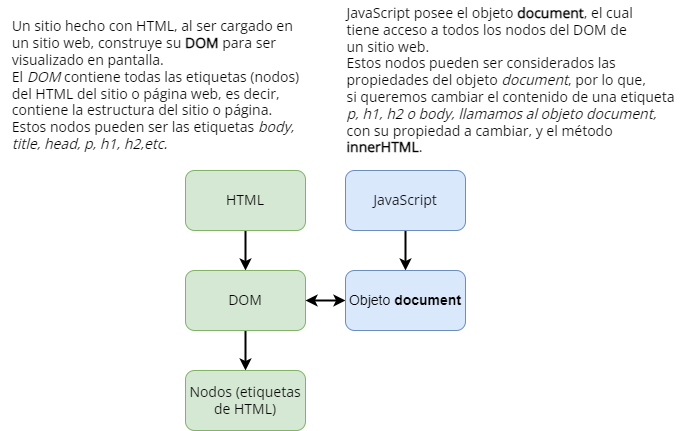
\includegraphics [width=13cm]{ss/dom_explicacion.png}
    \end{center}
\end{figure}

Presentamos también ejemplos de como se ve el uso del objeto \textbf{document} con las propiedades y métodos que posee:
\begin{lstlisting}
    // Declara variable que cambia el contenido de la etiqueta BODY.
    var cuerpo = document.body.innerHTML = "nuevo texto";
    // Declara variable que cambia el contenido de la etiqueta P.
    var parrafos = document.p.innerHTML = "NUEVO PARRAFO";
\end{lstlisting}

Basta con escribir el operador punto (.), seguido del nodo o etiqueta que queremos seleccionar, otro operador punto, y el método que queramos aplicar a la propiedad. \textbf{innerHTML()} es un método del objeto muy común de utilizar, cambia o devuelve el contenido de un nodo.


\subsection{Seleccionando elementos}

Entonces, \textbf{document} es un objeto que posee métodos y propiedades para interactuar con las propiedades de un sitio HTML, los siguientes métodos son los más utilizados para seleccionar elementos HTML:
\begin{lstlisting}
    // Encuentra un elemento por su ID.
    document.getElementById(id);
    // Encuentra un elemento por su nombre de etiqueta.
    document.getElementByClassName(nombre);
    // Encuentra un elemento por su etiqueta.
    document.getElementByTagName(etiqueta);
\end{lstlisting}

Volviendo a recordar HTML, sabemos que a una etiqueta podemos asignarle una clase o identificador, es por ello que los métodos anteriores buscan obtener uno o varios elementos a partir de la etiqueta que los representa, su identificador particular o clase:
\begin{lstlisting}
    <html>
        <head>
            <title>Prueba</title>
        </head>
        <body>
            <!-- Etiqueta con identificador -->
            <h1 id="cabecera">Hola mundo</h1>
            <!-- Etiqueta con clase asignada -->
            <p class="parrafos">Esto es un párrafo</p>
        </body>
    </html>
\end{lstlisting}

Por lo que, si utilizamos el método \textbf{getElementById()} o \textbf{getElementByClassName()} junto con \textbf{innerHTML}, podemos cambiar el contenido de las etiquetas con dicha clase e identificador:
\begin{lstlisting}
    <html>
        <head>
            <title>Prueba</title>
        </head>
        <body>
            <!-- Etiqueta con identificador -->
            <h1 id="cabecera">Hola mundo</h1>
            <!-- Etiqueta con clase asignada -->
            <p class="parrafos">Esto es un párrafo</p>
            
            <script>
                // Encuentra un elemento por su ID.
                var ej1 = document.getElementById("cabecera");
                ej1.innerHTML = "Hola mundo, nuevo texto.";
                // Encuentra un elemento por su nombre de etiqueta.
                var ej2 = document.getElementByClassName("parrafo");
                ej2[0].innerHTML = "Esto es un nuevo párrafo.";
            </script>
        </body>
    </html>
\end{lstlisting}

\textbf{getElementById} regresa únicamente un valor o elemento, ya que un identificador tiene la naturaleza de representar la identidad de un único elemento; \textbf{getElementByClassName} regresa una colección de datos (\textbf{un arreglo}), ya que múltiples etiquetas pueden estar modificados por una sola clase o varias, es por tal motivo que el código anterior tiene el operador llaves cuadradas con un índice.

\textbf{getElementByTagName} regresa también un arreglo con todos los elementos que tengan una etiqueta particular:
\begin{lstlisting}
    <html>
        <head>
            <title>Prueba</title>
        </head>
        <body>
            <p>hi</p>
            <p>hello</p>
            <p>hi</p>
            
            <script>
                // Encuentra un elemento por su etiqueta (p).
                var arr = document.getElementsByTagName("p");
                // Cambia el contenido de todos los elementos con etiqueta p.
                for (var x = 0; x < arr.length; x++) {
                    arr[x].innerHTML = "Hi there";
                }
            </script>
        </body>
    </html>

    /* Imprime:
    hi
    hello
    hi
    hi there
    hi there
    hi there
    */
\end{lstlisting}

La \textit{Tabla \ref{tab: 9}} contiene los métodos de los nodos para conocer su relación con otros nodos dentro del DOM:
\begin{table}[H]
    \begin{center}
        \caption{Métodos de nodos del objeto \textit{document}}
        \label{tab: 9}
        \begin{tabular}{c l}
            \hline
            \textbf{Método}&\textbf{Definición} \\
            \hline
            nodo.\textbf{childNodes}        & Regresa un arreglo con los nodos hijos del nodo \\
            nodo.\textbf{firstChild}        & Regresa el primer nodo hijo de un nodo \\
            nodo.\textbf{lastChild}         & Regresa el último nodo hijo de un nodo \\
            nodo.\textbf{hasChildNodes}     & Regresa true o false sin un nodo tiene hijos o no \\
            nodo.\textbf{nextSibling}       & Regresa el siguiente nodo del nodo actual en el mismo nivel \\
            nodo.\textbf{previosSibling}    & Regresa el nodo anterior del nodo actual en el mismo nivel \\
            nodo.\textbf{parentNode}        & Regresa el nodo padre del nodo actual \\
            \hline
        \end{tabular}
    \end{center}
\end{table}


\subsection{Cambiando elementos}

Ya vimos que con \textbf{innerHTML} podemos acceder o modificar el contenido de un nodo, ahora veremos que también podemos modificar las propiedades o atributos de los nodos:
\begin{lstlisting}
    <html>
        <head>
            <title>Prueba</title>
        </head>
        <body>
            <!-- Inserta una imagen y enlace -->
            <img id="mimg" src="banana.png"/>
            <a href="https://www.google.com">Esto es un enlace</a>
            
            <script>
                // Recibe el nodo con identificador "mimg".
                var el = document.getElementById("mimg");
                // Recibe arreglo con los nodos con etiqueta "a".
                var en = document.getElementByTagName("a");
                // Cambia la imagen y enlace de los respectivos nodos.
                el.src = "apple.png";
                en[0].href = "https://www.youtube.com";
            </script>
        </body>
    </html>
\end{lstlisting}

El estilo en cómo es presentado un nodo también se puede cambiar con JavaScript (color, fondo, alto, ancho, animación, etc). Todas las propiedades del lenguaje CSS pueden ser modificadas también con JavaScript, solamente recuerde que estas propiedades suelen utilizar mucho el guión (-) en sus nombres, por lo que, si desea cambiar una propiedad CSS con JavaScript, cree variables con el nombre de la propiedad, pero omitiendo el guión, dejando únicamente el nombre de la propiedad con mayúsculas y todo junto.
\begin{center}
    \textit{CSS: background-color\\JavaScript: backgroundColor}
\end{center}


\subsection{Agregando elementos}

Los métodos que aparecen en la \textit{Tabla \ref{tab: 10}} nos ayudarán a crear o eliminar nuevos y existentes nodos:
\begin{table}[H]
    \begin{center}
        \caption{Métodos para trabajar con nodos de \textit{document}}
        \label{tab: 10}
        \begin{tabular}{m{7cm} m{7cm}}
            \hline
            \textbf{Método} & \textbf{Definición} \\
            \hline
            nodo.\textbf{cloneNode()}                           & Clona un nodo \\
            document.\textbf{createElement(nodo)}               & Crea un nodo \\
            document.\textbf{createTextNode(texto)}             & Crea un nodo de solo texto \\
            nodo.\textbf{appendChild(nuevo nodo)}               & Agrega a un nodo otro nodo como último hijo \\
            nodo.\textbf{insertBefore(nodo1, nodo2)}            & Agrega a un nodo otro nodo1 hijo antes de otro nodo2 hijo \\
            nodo.\textbf{removeChild(nodo)}                     & Elimina un nodo hijo de un nodo padre \\
            nodo.\textbf{parentNode}                            & Regresa el nodo padre de un nodo \\
            nodo.\textbf{replaceChild(nodo1, nodo2)}    & Cambia un nodo por otro \\
            \hline
        \end{tabular}
    \end{center}    
\end{table}

Para los métodos que crean nodos, estos son creados pero no son adjuntados al DOM, por lo que deberán utilizar \textbf{appendChild()} o \textbf{insertBefore()} para poder adjuntarlos a la estructura HTML del sitio web:
\begin{lstlisting}
    <html>
        <head>
            <title>Prueba</title>
        </head>
        <body>
            <div id="prueba">Un texto</div>
            
            <script>
                // Crea un nuevo nodo "p".
                var p = document.createElement("p");
                // Crea un nodo solo de texto.
                var txt = document.createTextNode("Some new text");
                // Agrega el nodo solo texto al nodo "p".
                p.appendChild(node);
                // Recibe el nodo con identificador "prueba".
                var div = document.getElementById("prueba");
                // Agrega el nodo "p" al nodo con identificador "prueba".
                div.appendChild(p);
            </script>
        </body>
    </html>
\end{lstlisting}


\subsection{Eliminando elementos}

Si deseas eliminar un nodo del DOM, primero debes acceder a su nodo padre, utilizar el método \textbf{removeChild()}:
\begin{lstlisting}
    <html>
        <head>
            <title>Prueba</title>
        </head>
        <body>
            <!-- Crea un contenedor con identificador "demo" -->
            <div id="demo">
                <!-- Crea dos párrafos con identificador "p1" y "p2" -->
                <p id="p1">This is a paragraph.</p>
                <p id="p2">This is another paragraph.</p>
            </div>
            
            <script>
                // Recibe el nodo con identificador "demo".
                var padre = document.getElementById("demo");
                // Recibe el nodo con identificador "p1".
                var hijo = document.getElementById("p1");
                // Del nodo "padre" se elimina su nodo "hijo"
                padre.removeChild(hijo);
            </script>
        </body>
    </html>
\end{lstlisting}

En el ejemplo anterior, se elimina uno de los párrafos del contenedor div "demo". Podemos hacer esto de forma más directa con la propiedad \textbf{parentNode}:
\begin{lstlisting}
    padre.parentNode.removeChild(hijo);
\end{lstlisting}


\subsection{Reemplazando elementos}

Si requerimos quitar un nodo del DOM y poner otro para sustituirlo, podemos utilizar el método \textbf{replaceChild()}:
\begin{lstlisting}
    <html>
        <head>
            <title>Prueba</title>
        </head>
        <body>
            <!-- Crea un contenedor con identificador "demo" -->
            <div id="demo">
                <!-- Crea dos párrafos con identificador "p1" y "p2" -->
                <p id="p1">This is a paragraph.</p>
                <p id="p2">This is another paragraph.</p>
            </div>
            
            <script>
                // Crea un nuevo nodo "p".
                var p = document.createElement("p");
                // Crea un nodo solo texto.
                var nodo = document.createTextNode("This is new");
                // Asigna al nodo creado "p" el nodo solo texto ("p" con texto "This is new").
                p.appendChild(nodo);
                // Recibe el nodo con identificador "demo".
                var padre = document.getElementById("demo");
                // Recibe el nodo con identificador "p1".
                var hijo = document.getElementById("p1");
                // Remplaza el nodo hijo con el nuevo nodo "p".
                padre.replaceChild(p, hijo);
            </script>
        </body>
    </html>
\end{lstlisting}

Utiliza el mismo funcionamiento que el método anterior, donde primero debes seleccionar el nodo padre del nodo a reemplazar.



\section{Eventos}

Se puede ejecutar un bloque de código JavaScript cuando algo ocurre en el sitio web: un clic, el puntero encima de una etiqueta, recarga de la página, etc; a esto se le llama \textbf{evento}. La \textit{Tabla \ref{tab: 11}} contiene algunos de los eventos más comunes:
\begin{table}[H]
    \begin{center}
        \caption{Métodos para ejecutar eventos}
        \label{tab: 11}
        \begin{tabular}{m{3cm} m{10cm}}
            \hline
            \textbf{Evento} & \textbf{Definición} \\
            \hline
            onclick         & Ocurre cuando se da clic a un elemento \\
            onload          & Ocurre cuando un objeto ha sido cargado \\
            onunload        & Ocurre cuando una página no ha sido cargada (para $<$body$>$) \\
            windows.onload  & Realiza lo mismo que el evento onload \\
            onchange        & Ocurre cuando el contenido de un elemento de un \textit{form} ha cambiado (para $<$input$>$, $<$keygen$>$, $<$select$>$ y $<$textarea$>$) \\
            onmouseover     & Ocurre cuando el puntero está encima de un elemento o un hijo de este \\
            onmouseout      & Ocurre cuando el puntero sale de encima de un elemento o un hijo de este \\
            onmousedown     & Ocurre cuando el usuario presiona un botón del ratón encima de un elemento \\
            onmouseup       & Ocurre cuando el usuario deja de presionar un botón del ratón encima de un elemento \\
            onblur          & Ocurre cuando un elemento pierde el \textit{focus} \\
            onfocus         & Ocurre cuando un elemento obtiene el \textit{focus} \\
            onsubmit        & Ocurre cuando se envía un formulario \\
            \hline
        \end{tabular}
    \end{center}    
\end{table}


\subsection{Manejando eventos}

Los eventos son funciones de JavaScript, por lo que se los podemos asignar o adjuntar a una etiqueta en particular:
\begin{lstlisting}
    <html>
        <head>
            <title>Prueba</title>
        </head>
        <body>
            <!-- Etiqueta "p" que tiene un evento "onclick" asignado -->
            <p onclick="show()">Esto es un texto</p>
            
            <script>
                // Muestra un mensaje en pantalla con texto "Hola mundo".
                function show() {
                    alert("Hola mundo");
                }
            </script>
        </body>
    </html>
\end{lstlisting}

Así como hay dos formas de crear métodos de objetos, donde uno es hacerlo directamente en la declaración del objeto y el otro es adjuntarle la función al método en su declaración, con los eventos ocurre lo mismo:
\begin{lstlisting}
    <html>
        <head>
            <title>Prueba</title>
        </head>
        <body>
            <!-- Etiqueta "p" simple -->
            <p>Esto es un texto</p>
            
            <script>
                // Recibe los nodos con etiquetas "p".
                var x = document.getElementByTagName("p");
                // Al elemento 0 del arreglo con elementos "p" se el asigna la función onclick.
                x[0].onclick = function() {
                    // Despliega mensaje en sitio web.
                    alert("Hola mundo");
                }
            </script>
        </body>
    </html>
\end{lstlisting}


\subsubsection{Event Listeners}

Es la forma de agregar múltiples eventos a un solo nodo, su estructura es la siguiente:
\begin{lstlisting}
    nodo.addEventListener(evento, función, useCapture);
\end{lstlisting}

Donde:
\begin{itemize}
    \item \textbf{evento}: el evento que se desea ejecutar. No es necesario agregar el prefijo "\textbf{on}" al nombre del evento: onclick - click; onmouseover - mouseover.
    \item \textbf{función}: la función que el evento llamará cuando se ejecute.
    \item \textbf{useCapture}: parámetro con valor true y false, el primero para \textbf{bubbling} y el segundo para \textbf{capturing}.
\end{itemize}

Un ejemplo de los Event Listeners son:

\begin{lstlisting}
    <html>
        <head>
            <title>Prueba</title>
        </head>
        <body>
            <!-- Etiqueta "p" simple -->
            <p>Esto es un texto</p>
            
            <script>
                // Recibe los nodos con etiquetas "p".
                var x = document.getElementByTagName("p");
                // Agrega un Event Listener al nodo x.
                x[0].addEventListener("click", mifuncion());
                x[0].addEventListener("mouseover", mifuncion());
                // Muestra un mensaje en el sitio web.
                function mifuncion() {
                    alert("Hola mundo");
                }
            </script>
        </body>
    </html>
\end{lstlisting}

También se le quitar un Event Listener a un nodo, con el método \textbf{removeEventListener()}:
\begin{lstlisting}
    <html>
        <head>
            <title>Prueba</title>
        </head>
        <body>
            <!-- Etiqueta "p" simple -->
            <p>Esto es un texto</p>
            
            <script>
                // Recibe los nodos con etiquetas "p".
                var x = document.getElementByTagName("p");
                // Agrega un Event Listener al nodo x.
                x[0].addEventListener("click", mifuncion());
                // Muestra un mensaje en el sitio web y borra el Event Listener del nodo x.
                function mifuncion() {
                    alert("Hola mundo");
                    btn.removeEventListener("click", mifuncion);
                }
            </script>
        </body>
    </html>
\end{lstlisting}

\textit{Nota}: recuerde bien qué nodos poseen \textit{n} números de Event Listener y cuales son, para poder volver a utilizarlos o removerlos si son necesarios.


\subsection{Propagación de eventos}

Se refiere al orden o forma en la que un evento desencadena la ejecución de otros en la jerarquía del DOM del HTML: si se tiene un nodo "p" (hijo) dentro de un nodo "div" (padre), ambos tienen un evento \textit{onclick} y el usuario presiona el elemento "p", ¿cuál debería ejecutarse primero?, ¿el evento del padre o del hijo?

Cuando asignamos Event Listeners a nodos, uno de sus parámetros es \textbf{useCapture}, sus valores son:
\begin{itemize}
    \item \textbf{bubbling}: se ejecuta de abajo a arriba, de adentro a afuera, de hijo a padre. Su valor es false (por defecto).
    \item \textbf{capturing}: se ejecuta de arriba a abajo, de afuera a adentro, de padre a hijo. Su valor es true.
\end{itemize}
\begin{lstlisting}
    // Propagación capturing.
    nodo1.addEventListener("click", myFunction, true); 
    // Propagación bubbling.
    nodo2.addEventListener("click", myFunction, false);
\end{lstlisting}


\subsection{Validación con formulario}

HTML 5 ya posee el atributo \textbf{required} para sus formularios donde se requiere estrictamente que se llene algún elemento, pero JavaScript permite validación para profunda con su método \textbf{onsubmit}. Veamos el siguiente ejemplo:
\begin{lstlisting}
    <html>
        <head>
            <title>Prueba</title>
        </head>
        <body>
            <!-- Formulario con método "onsubmit" de JS -->
            <form onsubmit="return validar()" method="post">
                Número: <input type="text" name="num1" id="num1" />
                <br />
                Retítelo: <input type="text" name="num2" id="num2" />
                <br />
                <input type="submit" value="Envíar" />
            </form>
            
            <script>
                function validar() {
                    // Recibe los nodos con identificadores "num1" y "num2".
                    var n1 = document.getElementById("num1");
                    var n2 = document.getElementById("num2");
                    // Si ambos valores están vacíos.
                    if (n1.value != "" && n2.value != "") {
                        // Si ambos valores son iguales, regresa true.
                        if (n1.value == n2.value) {
                            return true;
                        }
                    }
                    // Lanza mensaje en sitio web y regresa false.
                    alert("The values should be equal and not blank");
                    return false;
                }
            </script>
        </body>
    </html>
\end{lstlisting}

\textit{Nota}: si la función regresa false, el formulario no se envía.

Tenemos un formulario que recibe dos números, donde el objetivo es que ambos números sean iguales para enviar el formulario. Para lograr esto, utilizamos la función "validar" de JS, donde primero evalúa si los dos valores están vacíos: si es el caso, no envía el formulario; si los dos valores si tuviesen contenido, evalúa si son iguales: si lo son, regresa true, sino, regresa el mismo resultado que el caso de que ambos valores estuviesen vacíos. Con esto, obtenemos la validación de datos de un formulario con JS.

\section{ECMAScript 6}
\hspace{0.55cm}ECMAScript 6 (ahora abreviado ES6), y posteriormente llamado ECMAScript 2015, es una de las versiones más populares de JavaScript. Esta versión buscó estandarizar el lenguaje, trayendo consigo muchas nuevas funciones y herramientas, como: nueva sintaxis, clases, módulos, iteradores para ciclos, generadores, datos binarios, arreglos \textit{tipado}s, nuevas colecciones de datos (mapas, mapas débiles y Sets), \textit{promesas}, mejoras para los tipos números y matemáticas \textit{reflection}, \textit{proxies}, etc.


\subsection{Variables y cadenas}
\hspace{0.55cm}Antes de mencionar los tipos de variables en esta versión de JavaScript, mencionemos el concepto \textbf{Scope:}


\subsubsection{Scope}
\hspace{0.55cm}El \textbf{Scope} (\textbf{Alcance, Límite, Enfoque}) en los lenguajes de programación es el área donde una variable u objeto tiene validez, puede interactuar con otras variables y es útil: una variable puede tener un Scope únicamente al bloque true o false de una condicional, al bloque en bucle de un ciclo, al bloque de instrucciones de una función o de una clase.

Podemos declarar variables de tres maneras:
\begin{itemize}
    \item \textbf{var}: son variables globales o con un Scope un poco más general.
    \item \textbf{const}: son variables que no pueden cambiar su valor, una vez se le asigna uno, ya no puede cambiar.
    \item \textbf{let}: son variables con un Scope muy reducido.
\end{itemize}

\subsubsection{Template Literals}
\hspace{0.55cm}La nueva forma de poder desplegar variables en esta versión del lenguaje es la siguiente:
\begin{center}
    \textit{
            // Declara variable.
            let nombre = "David";
            // Forma de desplegar.
            console.log("Bienvenido " + nombre);
            // Nueva forma de desplegar.
            console.log(`Bienvenido \$\{nombre\}`);
            }
\end{center}

Fíjese que el ejemplo donde se utiliza el símbolo de dinero (\$) y un par de llaves (\{\}) se encierra el texto a mostrar dentro de comillas inversas (``), esto debido a que el formato \textbf{\$\{expresión\}} es un \textbf{marcador de posición}.


\subsection{Ciclos y funciones}


\subsubsection{Nueva sintaxis de funciones y parámetros predeterminados}
\hspace{0.55cm}Podemos volver atrás en este documento para poder recordar como declarar una función, sin embargo, esta versión de JS tiene una nueva sintaxis para la declaración de métodos:
\begin{lstlisting}
    // Vieja sintaxis.
    function suma(num1, num2) {
        suma = sum1 + sum2;
        console.log(`La suma es: ${suma}$`);
    }
    // Nueva sintaxis.
    const suma = (num1, num2) => {
        suma = sum1 + sum2;
        console.log(`La suma es: ${suma}$`);
    }
\end{lstlisting}

Esta nueva sintaxis puede adaptarse a funciones que no poseen parámetros no solamente tiene uno:
\begin{lstlisting}
    // Regresa el cuadrado de un número.
    const cuadrado = x => x * x;
    // Regresa un mensaje en el sitio web.
    const mensaje = () => alert("Hola mundo");
\end{lstlisting}

Vemos que la simplificación de la nueva sintaxis es considerable para funciones con una instrucción y uno o ningún parámetro, si requieres regresar un valor de la función con la palabra reservada \textbf{return} con la nueva sintaxis, utilizar esta palabra no será necesaria.

Podemos crear parámetros con valores por defecto en nuestras funciones:
\begin{lstlisting}
    // Regresa la suma de un parámetro con los otros dos predeterminados.
    const suma = (a, b=3, c=4) => {
        return a + b + c;
    }
    // Regresa la multiplicación de dos parámetros predeterminados con uno regular
    const multi = (a=2, b, c=3) => {
        return a * b * c;
    }

    // Imprime la llamada a las funciones.
    console.log(suma(1));
    console.log(multi(2));

    /*
    Imprime:
    8
    12
    */
\end{lstlisting}

Los parámetros de las funciones suelen ser recorridos de izquierda a derecha, también, si deseamos cambiar uno de los valores de los parámetros predeterminados, el lenguaje nos lo permite.

Se integra a los tipos de ciclos válidos en el lenguaje los ciclos \textbf{For...in} y \textbf{For...of}.


\subsubsection{Ciclo For...in}
\hspace{0.55cm}Este ciclo es utilizado para iterar sobre las llaves de objetos, no para arreglos, esto debido a que la variable contador es de tipo cadena, contrario a los índices de un arreglo, el cual es un entero. Veamos un ejemplo:
\begin{lstlisting}
    // Declara tupla.
    let obj = [a:1, b:2, c:3, d:4];
    // Imprime sus llaves por medio de ciclo For..in.
    for (let v in obj) {
        console.log(v);
    }

    /*
    Imprime:
    a
    b
    c
    */
\end{lstlisting}

Lo que se desplegará son las llaves de una colección tupla.

\subsubsection{Ciclo For...of}
\hspace{0.55cm}Este ciclo es utilizado para iterar sobre objetos iterables (\textit{arreglos, Map, Set, WeakMap} y \textit{WeakSet}) por medio de una variable que adopta el tipo de dato según el tipo de dato que maneje la colección. Veamos un ejemplo:
\begin{lstlisting}
    // Declara un arreglo.
    let obj = ["a", "b", "c", "d"];
    // Imprime sus elementos por medio del ciclo For...of.
    for (let v of obj) {
        console.log(v);
    }
    // Imprime los caracteres de la cadena por medio del ciclo For...of.
    for (let v of "Hola") {
        console.log(v);
    }

    /*
    Imprime:
    a
    b
    c
    H
    o
    l
    a
    */
\end{lstlisting}



\subsection{Objetos ES6}
\hspace{0.55cm}La nueva versión del lenguaje te permite escribir menos a la hora de declarar métodos de objetos e inicializar sus propiedades:
\begin{lstlisting}
    // Declara objeto.
    let arbol = {
        // Declara atributos del objeto.
        altura: 10,
        color: "verde",
        // Declara, de forma reducida, un método del objeto.
        crecer() {
            this.altura += 2;
        }
    };
    // Declara variables para inicializar propiedades de un objeto.
    let nombre = "mario";
    let edad = 21;
    // Declara objeto.
    let atleta = {
        // Utiliza variables para inicializar propiedades.
        nombre,
        edad
    };
    // Llamada al método para hacer crecer al árbol.
    arbol.crecer();
    console.log(arbol.altura);

    // Imprime: 12
\end{lstlisting}

En caso de crear un objeto con múltiples propiedades con el mismo nombre y distintos valores, la última propiedad con el mismo nombre sobre escribirá el resto:
\begin{center}
    \textit{
            // Imprime: 4 \\
            var a = {x: 1, x: 2, x: 3, x: 4};
            }
\end{center} 


\subsubsection{Nombres computados para propiedades}
\hspace{0.55cm}Los \textbf{nombres computados para propiedades} son nombres construidos a partir de otras variables, con el operador corchetes cuadrados (\textbf{[]}) dentro de un objeto de clase, obtenemos este resultado:
\begin{lstlisting}
    // Declara variables.
    let nombre = "nombre";
    let id = 1234;
    let num_tel = 5546788876;
    var i = 0;
    // Declara objeto.
    let usuario = {
        // Declara nombre de propiedad según el contenido de la variable "nombre".
        [nombre]: "luis",
        // Declara nombre de propiedad según el texto "usuario_" y el contenido de la variable "id".
        [`usuario_${id}`]: `${num_tel}`
    }
    // Declara objeto.
    var a = {
        // Declara nombre de propiedad según el contenido de la variable "i".
        ['foo' + ++i]: i,
        ['foo' + ++i]: i,
        ['foo' + ++i]: i
    };
    // Imprime valores de propiedades
    console.log(user.name);
    console.log(user.user_1234);
    console.log(a.foo1);
    console.log(a.foo2);
    console.log(a.foo3);

    /*
    Imprime:
    luis
    1234
    1
    2
    3
    */
\end{lstlisting}


\subsubsection{Objet.assign()}
\hspace{0.55cm}Es un nuevo método de los objetos que permite crear o asignar a un objeto las propiedades de otros objetos, con este método, podemos crear nuevos objetos o duplicar otros:
\begin{lstlisting}
    // Declara objeto.
    let person = {
        name: 'Jack',
        age: 18,
        sex: 'male'
    };
    // Declara objeto.
    let student = {
        name: 'Bob',
        age: 20,
        xp: '2'
    };
    // Declara objeto construido a partir de las propiedades de los objetos "person" y "student".
    let newStudent = Object.assign({}, person, student);
    // Imprime los valores de las propiedades.
    console.log(newStudent.name); // Bob
    console.log(newStudent.age); // 20
    console.log(newStudent.sex); // male
    console.log(newStudent.xp); // 2
\end{lstlisting}

El primer parámetro con las llaves vacías es el objeto destino, y después de este, el resto de parámetros son los objetos con los que se construirá otro, podemos utilizar tantos objetos como queramos. Debemos tomar en cuenta el orden de como vamos escribiendo los objetos a utilizar ya que, si dos o más objetos tienen propiedades con el mismo nombre, el último objeto con dichas propiedades sobre escribirá al resto, en el ejemplo anterior, vemos que el objeto "person" y "student" poseen dos propiedades con el mismo nombre (name y age), sin embargo, los valores de las propiedades con el mismo nombre del objeto "newStudent" son "Bob" y "20", en vez de ser "Jack" y "18"; pruebe cambiar el orden de los objetos en la declaración de newStudent para ver cuales serán los valores de sus propiedades.

Se podría pensar que con utilizar el operador de igual (=) se puede duplicar un objeto:
\begin{center}
    \textit{nuevoObjecto = objecto;}
\end{center}

Esto generaría una \textbf{referencia} al objeto original, es como un acceso directo en los sistemas operativos, si se cambian los valores en la referencia, el objeto original también recibirá los cambios:
\begin{lstlisting}
    // Declara objeto.
    let person = {
        name: 'Jack',
        age: 18
    };
    // Declara objeto con referencia a "person".
    let newPerson = person;
    // Cambia el valor de la propiedad del objeto referencia.
    newPerson.name = 'Bob';
    // Imprime las propiedades "name" de ambos objetos.
    console.log(person.name);
    console.log(newPerson.name);

    /*
    Imprime:
    Bob
    Bob
    */
\end{lstlisting}

Con el método assign(), podemos crear un objeto a partir de las propiedades de otro, pudiendo cambiar el valor de una de las propiedades a recibir:
\begin{lstlisting}
    // Declara objeto.
    let person = {
        name: 'Jack',
        age: 18
    };
    // Declara objeto con referencia a "person".
    let newPerson = Objet.assign({}, person, {name:"Bob"});
    // Imprime las propiedades "name" de ambos objetos.
    console.log(newPerson.name);

    /*
    Imprime:
    Bob
    */
\end{lstlisting}


\subsection{Clases}
\hspace{0.55cm}Para declarar una clase en ES6, se utiliza la palabra reservada \textbf{class}, y para crear objetos de clases es requerido utilizar la palabra reservada \textbf{new}:
\begin{lstlisting}
    // Declara clase.
    class Rectangulo {
        // Constructor que inicializa atributos de clase.
        constructor(ancho, altura) {
            this.ancho = ancho;
            this.altura = altura;
        }
        // Regresa el cálculo del área.
        area() {
            return this.calcArea();
        }
        // Calcula el área del rectángulo.
        calcArea() {
            return this.ancho * this.altura;
        }
    }
    // Declara objeto de clase Rectangulo.
    const rect = new Rectangulo(5, 6);
    // Imprime: 30.
    console.log(rect.area());
\end{lstlisting}

Algo que no se ha mencionado a lo largo de este documento, es que \textbf{las funciones en JS pueden ser llamadas sin haber sido declaradas anteriormente}, a diferencia de otros lenguajes donde es requerido que declares una una función previo a llamarla; las clases en JS si deben ser declaradas antes de utilizarlas, no como las funciones.


\subsubsection{Constructores}
\hspace{0.55cm}Aquí también tenemos presente los \textbf{constructores}, el cual puede ser instanciado o no dentro de la declaración de una clase, su principal característica es que \textbf{solamente puede haber un constructor por clase}, no como en otros lenguajes, donde estos pueden ser sobrecargados.
\begin{center}
    \textit{constructor(parámetros) \{ //Instrucciones. \}}
\end{center}


\subsubsection{Tipos de clases}
\hspace{0.55cm}Además de las clases regulares, que acabamos de ver, existen las \textbf{clases nombradas} y \textbf{sin nombrar}, estas son el producto de las \textbf{expresiones de clases}, como vemos enseguida:
\begin{lstlisting}
    // Declara clase nombrada.
    var rect = class Rectangulo {
        constructor(ancho, altura) {
            this.ancho = ancho;
            this.altura = altura;
        }
    }

    // Declara clase sin nombrar.
    var rect = class {
        constructor(ancho, altura) {
            this.ancho = ancho;
            this.altura = altura;
        }
    }
\end{lstlisting}

Como podemos observar, una clase nombrada es una clase con nombre en la declaración que es asignada a una variable (let, const o var), mientras que una clase no nombrada es una clase sin nombre en la declaración; podemos ver a este tipo de clases como saltarnos el paso de declarar la clase y luego su objeto:
\begin{lstlisting}
    // Declara clase de forma regular.
    class Rectangulo {
        constructor(ancho, altura) {
            this.ancho = ancho;
            this.altura = altura;
        }
        area() {
            return this.calcArea();
        }
        calcArea() {
            return this.ancho * this.altura;
        }
    }
    // Declara objeto de clase Rectangulo de forma regular.
    const rect = new Rectangulo(5, 6);

    // Declara clase nombrada en una variable, omitiendo la declaración
    // de la clase y del objeto.
    var rect = class Cuadrado {
        constructor(lado) {
            this.lado = lado;
        }
    }
\end{lstlisting}


\subsubsection{Tipos de métodos}
\hspace{0.55cm}Los \textbf{métodos prototipo} son las funciones a las que los objetos de clases pueden acceder; son los métodos que utilizamos todo el tiempo en en las clases. Este tipo de métodos no requiere de alguna palabra reservada particular.

Los \textbf{métodos estáticos} son las funciones que únicamente pueden acceder directamente una clase, no sus objetos, esto con el objeto de limitar el alcance y uso del método. Este tipo de métodos requiere de la palabra reservada \textbf{static}, previo al nombre del método, para ser declarado.
\begin{lstlisting}
    // Declara clase de forma regular.
    class Rectangulo {
        constructor(ancho, altura) {
            this.ancho = ancho;
            this.altura = altura;
        }
        area() {
            return this.ancho * this.altura;
        }
        perimetro() {
            return (this.ancho * this.altura) / 2;
        }
        // Método estático que recibe otro objeto Rectangulo como parámetro, imprime sus atributos más dos.
        static sumar_valores(a) {
            a.ancho += 2;
            a.altura += 2;
            console.log(a.ancho + ", " + a.altura);
        }
    }
    // Declara objeto de clase Rectangulo de forma regular.
    const rect = new Rectangulo(5, 6);
    // Llamada al método estático de la clase Rectangulo.
    Rectangulo.sumar_valores(rect);
\end{lstlisting}


\subsubsection{Herencia}
\hspace{0.55cm}La palabra reservada \textbf{extends} es utilizada para heredar el contenido de una clase a otra:
\begin{lstlisting}
    // Declara clase base.
    class Animal {
        // Constructor.
        constructor(name) {
            this.name = name;
        }
        // Método que imprime un mensaje.
        speak() {
            console.log(this.name + ' makes a noise.');
        }
    }
    // Declara clase derivada.
    class Dog extends Animal {
        // Método de clase basee que imprime un mensaje.
        speak() {
            // Llama al método de la clase base.
            super.speak(); // Super
            // Imprime mensaje.
            console.log(this.name + ' barks.');
        }
    }
    // Declara objeto de clase Dog.
    let dog = new Dog('Rex');
    // Llamada al método que imprime mensaje.
    dog.speak();

    /*
    Imprime:
    Rex makes a noise.
    Rex barks.
    */
\end{lstlisting}

Nótese que se está utilizando el método \textbf{super()}, el cual es un acceso directo a los métodos y atributos de la clase base de la clase derivada.


\subsection{Desempacando arreglos y objetos}
\hspace{0.55cm}Así como en Python, podemos asignarle a múltiples variables los elementos de un arreglo o las propiedades de un objeto:
\begin{lstlisting}
    // Declara arreglo.
    let arreglo = [1, 2, 3];
    // Declara objeto.
    let objeto = {
        prop1: 100,
        prop2: true
    };
    // Asigna a múltiples variables los elementos de un arreglo.
    let [num1, num2, num3] = arreglo;
    // Asigna a múltiples variables las propiedades de un objeto.
    let {prop1, prop2} = objeto;
    // Imprime valores.
    console.log(prop1);
    console.log(prop2);
    console.log(num1);
    console.log(num2);
    console.log(num3);

    /*
    Imprime:
    100
    true
    1
    2
    3
    */
\end{lstlisting}

Tome en cuenta que las variables que recibirán las variables de las propiedades de un objeto tendrán el mismo nombre que las propiedades, en el ejemplo anterior, el objeto "objeto" tiene las propiedades "prop1" y "prop2", y las variables que reciben sus valores son llamadas de la misma manera. Considere la existencia de elementos con valores predeterminados en los elementos de los arreglos:
\begin{lstlisting}
    // Declara variables.
    let a, b, c = 4, d = 8;
    // Asigna a la variable "a" el valor "2", "b" se mantiene con su valor por defecto.
    [a, b = 6] = [2];
    // Se intercambian los valores de las variables.
    [c, d] = [d, c];

    console.log(a);
    console.log(b);
    console.log(c);
    console.log(d);

    /*
    Imprime:
    2
    6
    8
    4
    */
\end{lstlisting}

En caso de que se le quieran asignar los valores de las propiedades de un objeto a múltiples variables que a fueron declaradas, la sintaxis cambia un poco:
\begin{lstlisting}
    // Declara variables.
    let a, b;
    // Asigna a variables las propiedades de un objeto.
    ({a, b} = {a: "hola", b: "mundo"});
    // Imprime resultados.
    console.log(a + b);

    // Imprime: hola mundo.
\end{lstlisting}

Si deseamos cambiar el nombre de las variables que recibirán los valores de las propiedades de un objeto, utilizamos la siguiente sintaxis:
\begin{lstlisting}
    // Declara objeto.
    let objeto = {prop1: 100, prop2: true};
    // Asigna a variables "p1" y "p2" las propiedades del objeto "objeto".
    let {prop1: p1, prop2: p2} = objeto;
    // Despliega valores.
    console.log(prop1);
    console.log(p1);

    /*
    Imprime:
    Error
    100
    */
\end{lstlisting}


\subsection{Rest \& Spread}
\hspace{0.55cm}Así como con Python, este lenguaje permite que una función pueda recibir \textit{n} cantidad de parámetros en una llamada, otra cantidad en otra llamada, así cuantas veces requerimos, podemos llamar a esto \textbf{parámetros variables}, esto lo obtenemos con la sentencia \textbf{arguments}:
\begin{lstlisting}
    // Declara función con un parámetro, que es una lista.
    function ejemplo(arr) {
        // Ciclo para recorrer los elementos del parámetro variable "arguments".
        for (let i = 1; i < arguments.length; i++) {
            // Declara variable que va recibindo los elementos del parámetro variable "arguments".
            let num = arguments[i];
            // Si la variable anterior no está presente en el arreglo, regresa falso.
            if (arr.indexOf(num) == -1) {
                return false;
            }
        }
        return true;
    }
    
    let x = [2, 4, 6, 8];
    // Llamada a la función con distintos valores en los parámetros.
    console.log(ejemplo(x, 2, 4 ,7));
    console.log(ejemplo(x, 6, 4, 9));

    /*
    Imprime:
    true
    false
    */
\end{lstlisting}

En cambio, SE6 introduce la nueva sentencia para utilizar los parámetros variables: los parámetros \textbf{Rest} son los famosos parámetros variables y pueden ser nombrados como queramos, además, requieren del \textbf{operador tres puntos} (\textbf{...)}; veamos un ejemplo:
\begin{lstlisting}
    // Declara función con un parámetro, que es una lista.
    function ejemplo(arr, ...nums) {
        // Ciclo For...of para recorrer el parámetro Rest.
        for (let num of nums) {
            // Si la variable anterior no está presente en el arreglo, regresa falso.
            if (arr.indexOf(num) === -1) {
                return false;
            }
        }
        return true;
    }
    // Declara arreglo.
    let x = [2, 4, 6, 7];
    // Llamada a la función con distintos valores en los parámetros.
    console.log(ejemplo(x, 2, 4 ,7));
    console.log(ejemplo(x, 6, 4, 9));

    /*
    Imprime:
    true
    false
    */
\end{lstlisting}

En caso de que el parámetro Rest solamente reciba un elemento, en vez de un conjunto de elementos, dentro de la función, la lista de elementos solamente tendrá un valor (índice 0).

Apuntes sobre Spread se realizarán más adelante.


\subsection{Map y Set}
\hspace{0.55cm}Un objeto \textbf{Map} puede contener pares de llaves y valores, como las duplas de Python u otros lenguajes, las llaves y valores pueden ser tipos de datos primitivos, objetoso o funciones.

Un objeto Map puede ser inicializado con iterables, donde cada par de corchetes cuadrados representa un arreglo de dos posiciones u otro tipo de iterable:
\begin{lstlisting}
    let mapa = new Map([
    [iterable1],
    [iterable2],
    .
    .
    .
    [iterableN]
    ])
\end{lstlisting}

Un objeto Map es diferente a un objeto regular debido a los siguientes puntos:
\begin{enumerate}
    \item Las llaves pueden ser cualquier tipo de dato (primitivo, funciones u otros objetos).
    \item Puedes obtener el tamaño del mapa.
    \item Puedes iterar directamente en un mapa.
    \item El funcionamiento de los mapas es mejor cuando se tiene una situación donde se está constantemente agregando, cambiando o eliminando valores con llaves.
\end{enumerate}

Los métodos de los mapas vienen en la \textit{Tabla \ref{tab: 12}}:
\begin{table}[H]
    \begin{center}
        \caption{Métodos del objeto Map}
        \label{tab: 12}
        \begin{tabular}{m{3cm} m{10cm}}
            \hline
            \textbf{Método} & \textbf{Definición} \\
            \hline
            set(llave, valor)   & Agrega una nueva llave y su valor al mapa. Si la llave la existe, sustituye su valor en el mapa con el que se desea agregar \\
            get(llave)          & Regresa el valor correspondiente a la llave solicitada. Si la llave no existe, regresa \textbf{undefined} \\
            has(llave)          & Regresa \textit{true} si la llave solicitada existe, \textit{false} en caso contrario \\
            delete(llave)      & Elimina la llave y valor del mapa según la llave solicitada y regresa \textit{true}; regresa \textit{false} si la llave no existe \\
            clear()             & Elimina todas las llaves y sus valores del mapa \\
            keys()              & Regresa un iterador con todas las llaves de un mapa \\
            values()            & Regresa un iterador con todos los valores de un mapa \\
            entries()           & Regresa un iterador con un arreglo con todas las llaves y valores de un mapa \\
            \hline
        \end{tabular}
    \end{center}    
\end{table}

Veamos un ejemplo ahora de los mapas y sus métodos:
\begin{lstlisting}
    // Declara un objeto Map vacío.
    let mapa = new Map();
    // Agrega varios pares al mapa.
    mapa.set("1", 1);
    mapa.set("2", 2);
    mapa.set("3", 3).set("4", 4);
    // Imprime los valores de las llaves "1" y "2".
    console.log(mapa.get("1"));
    console.log(mapa.get("2"));
    // Elimina la llave "4" y su valor.
    console.log(mapa.delete("4"));
    // Verifica si existe la llave "4" en el mapa.
    console.log(mapa.has("4"));
    // Imprime, por medio del método "entries()", los pares del mapa.
    for (let i of mapa.entries()) {
        console.log(i[0] + " : " + i[1]);
    }

    /*
    Imprime:
    1
    2
    true
    false
    1 : 1
    2 : 2
    3 : 3
    */
\end{lstlisting}

Los objetos \textbf{Set} son un tipo de arreglo donde solo se almacenan valores \textbf{únicos}, es decir, no se puede repetir un elemento dentro del conjunto; estos valores pueden ser tipos primitivos u otros objetos.

Un objeto Set puede ser inicializado con iterables, donde cada par de corchetes cuadrados representa un arreglo de dos posiciones u otro tipo de iterable:
\begin{lstlisting}
    let conjunto = new Set([
    [iterable1],
    [iterable2],
    .
    .
    .
    [iterableN]
    ])
\end{lstlisting}

Los métodos de los conjuntos vienen en la \textit{Tabla \ref{tab: 13}}:
\begin{table}[H]
    \begin{center}
        \caption{Métodos del objeto Set}
        \label{tab: 13}
        \begin{tabular}{m{3cm} m{10cm}}
            \hline
            \textbf{Método} & \textbf{Definición} \\
            \hline
            add(valor)      & Agrega un elemento al conjunto \\
            delete(valor)   & Elimina un elemento específico del conjunto \\
            has(valor)      & Regresa \textit{true} si un elemento existe dentro del conjunto, regresa \textit{false} si no se encuentra \\
            clear()         & Elimina todos los elementos del conjunto \\
            values()        & Regresa un iterador con todos los elementos del conjunto \\
            \hline
        \end{tabular}
    \end{center}    
\end{table}

Veamos un ejemplo ahora de los conjuntos y sus métodos:
\begin{lstlisting}
    // Declara un objeto Set vacío.
    let con = new Set();
    // Agrega varios valores al conjunto.
    con.add(5);
    con.add(9);
    con.add(59);
    con.add(9).add(5).add(59).add(60);
    // Elimina el valor 60.
    con.delete(60);
    // Verifica si existe el valor 60 en el conjunto.
    con.has(60)
    // Imprime, por medio del método "values()", los valores del conjunto.
    for (let i of con.values()) {
        console.log(i);
    }
    
    Imprime:
    false
    5
    9
    59
    */
\end{lstlisting}

Veamos que se agregaron más de una vez el valor "5", "9" y "59", sin embargo, no fueron repetidos dentro del conjunto.

% Fin del documento.
\end{document}